
\section{Technical background}
\label{sec:technical_background}

The software used in this project employ many different and important techniques known from distributed computing, which will be discussed here.
In section \ref{sec:consistenthashing} we will talk about the key aspect consistent hashing.
We will then discuss how consistent hashing techniques help us build \emph{available} and \emph{durable} databases.

Section \ref{sec:failures} discusses how failures are handled in the system. The tunability of the database is introduced in section \ref{sec:tunability}.

We lastly introduce PAXOS, a protocol for reaching consensus in a set of independent nodes.

\subsection{Consistent hashing}
\label{sec:consistenthashing}
Consistent hashing is a technique introduced in 1997 by David Karger\cite{Karger97consistenthashing} et al.
The technique is used to solve problems with locating a key in a distributed system.
Assume you have $n$ servers in the system, then number these from $0$ to $n-1$.
The \emph{hashspace} of the keys are then divided into $n$ partitions. Then, to find which server to put a key on, do a $$\textrm{Hash(key) mod } n$$ and you have the server number for the key. 

However, with this scheme if a server fails and you now have $n-1=m$ servers, all the failed server's data is gone.
You have to invalidate all existing servers, renumber your set of servers and start over.
Analogously, if you add $k$ servers to accommodate higher traffic, you now have $$\textrm{Hash(key) mod } n + k$$ and it is easy to see that all or most keys will have to relocate.

Consistent hashing reduces this problem by assigning each node with a number of points in the hash space.
The hash space is viewed as a ring by wrapping around \texttt{0000-FFFF}. The nodes are placed at points along the ring as in Figure \ref{fig:hashring}. When a key is looked up, you find it's place on the ring and move clockwise to the first point with an assigned node. In Figure \ref{fig:hashring}, key K is routed to the next node on the ring, node B.

Now remember we let the nodes take on \emph{several} points along the ring, thus spreading a nodes responsible key space to smaller pieces along the ring.
I.e. nodes B, E and G in Figure \ref{fig:hashring} could be the same \emph{physical} node.

\begin{figure}[h]
    \centering
    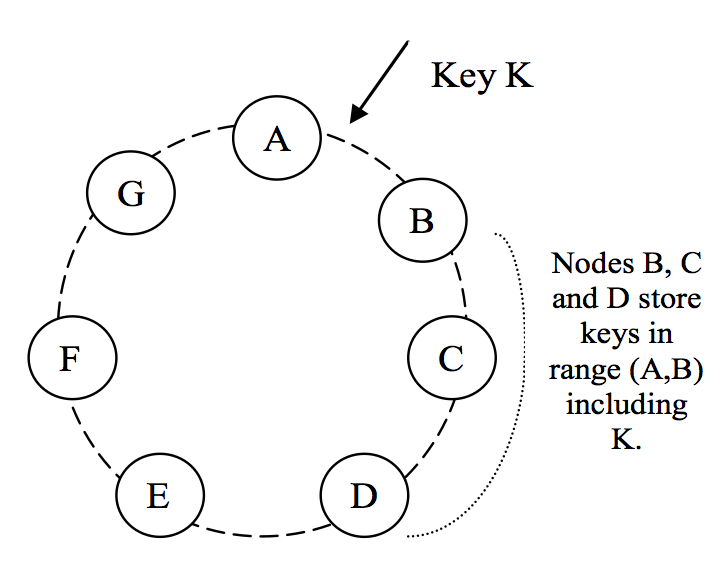
\includegraphics[width=0.5\textwidth]{background/figures/hashring}
    \caption{Hash ring with several nodes\cite{dynamo}.}
    \label{fig:hashring}
\end{figure}

This approach to locating keys has several advantages:

\begin{itemize}
\item Like before, we distribute operations on the set of available servers. By having each server take numerous positions on the hash ring, we also gain a more even distribution of the amount of key space among the nodes, compared to giving them a single random or fixed position.

\item Consistent hashing can also accommodate different types of servers by allowing more powerful nodes to have more points assigned on the ring, and vice versa. 

\item When adding a new server, a number of different areas around the circle are affected, and not one contiguous piece. This means the work of adding in the new node will be spread over the system, and not all requests routed to a single node.

\item The spread of the key space also avoids rehashing of more than $k/n$ keys when adding a new node. 

\item When a node fails, you move along the ring to the next server. When the nodes occupy several points on the ring, the extra work because of a failing node will be distributed among all the nodes in the system.
\end{itemize}

Consistent hashing also conveniently allows for easy, tunable replication of data to ensure durability, as used by key-value stores Dynamo\cite{dynamo} and Voldemort\cite{voldemort}. Consider W the number of data replicas to create. Hash the key, then move along the ring, writing key K to the W first nodes encountered on the ring. This will also ensure backups to be available along the ring when a node fails and requests gets passed along.

\subsection{Durability}
As explained in \ref{sec:consistenthashing}, both Voldemort and Dynamo use consistent hashing to locate and store keys.
They are both key-value stores only.
The goals for the Voldemort project is a database which is highly available and fault tolerant, providing an \emph{always-on} experience.

To safely store user data, redundancy is required. 
The typical approach to this is synchronously storing replicas at different locations to ensure data replication. 
In practice though, providing this kind of strong consistency in a database system can prove detrimental to availability in some failure scenarios.
A common approach to failure is locking down data and making it unavailable until the failure is resolved, so as not to serve potentially stale or erroneous data.
While it is convenient for the programmer to never have to deal with possibly failed data, locking down doubtful data is not ideal for performance.
In distributed systems network and system failures can be quite common, making guarantees of strong consistency very costly. In practice, strong consistency can be considered incompatible with high availability.
This makes traditional replication methods unsuitable for highly concurrent distributed systems.

\begin{wrapfigure}{R}{0.5\textwidth}
    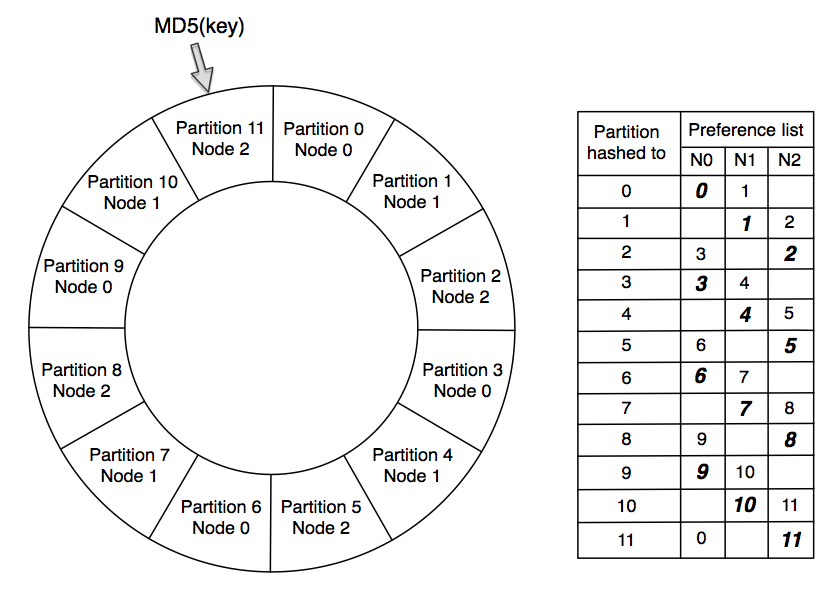
\includegraphics[width=0.5\textwidth]{background/figures/hashring_voldemort}
    \caption{Hash ring with 3 nodes and 12 partitions from Voldemort\cite{dynamo} with N=2. Partitions are a fixed number of splits of the keyspace. Nodes are assigned a number of partitions which they hold. When a request is routed, one first hashes the key to find the partition the key belongs on. One then asks nodes in the order of the \emph{preference list} for the key.}
    \label{fig:voldemort_hashring}
\end{wrapfigure}

To help provide higher availability of data, an optimistic approach to replication is used.
By allowing replicas to gradually propagate in the background and not synchronously, the workload on a distributed database system is greatly relieved, allowing for higher throughput. By also allowing conflicting data, we can continue to serve data in times of failure. This will cause more work for the application developers, and they need to be aware of this when using the database. Allowing conflicts also helps availability of put operations, and allows us the possibility to always accept a write.

It is easy to see how the consistent hashing ring helps implement this approach in Voldemort.
To ensure data durability, one can simply write the data to the next few nodes on the ring. In Dynamo and Voldemort this is a tunable parameter, W, which controls how many nodes a write synchronously has to reach to be successful. 
Internally it is called \emph{required writes}.

Similarly, it is easy to see how we can implement optimistic replication:
By allowing nodes to push written objects in the background, at a later time, to any number of nodes further down the ring.
This number \emph{N}, is called the \emph{replication factor}, and designates the number of replicas we \emph{eventually} want to be present.
I.e. we will have an \emph{eventually consistent} form of replication.

You should also note that this replication has two benefits: 
\begin{itemize}
	\item As a data backup should the other node have a hard drive failure.
	\item As a functional backup. If the other node is off line, the replica can take over the workload with all the data available.
\end{itemize}

In Voldemort, the hash ring is split into X equally sized parts, called \emph{partitions}. Each partition is assigned a unique ID and maps to a node.
The nodes create a \emph{preference list} over the partitions, which says to which \emph{partitions} it should store the replicas.

Now let $N=2$ with 12 partitions as in Figure \ref{fig:voldemort_hashring}. 
Let a key K's hash belong in partition 0. From the preference list, we see that this key should be put in \texttt{node0}, and replicated to the node holding partition 1, which is \texttt{node1}.
Voldemort also does some sanity checking when replicating, such that replicas are always replicated to N \emph{physical} nodes. 
I.e. In our example, if both partition 0 and 1 where held by \texttt{node0}, Voldemort would move along the ring until it finds the next partition that is assigned to a different node before storing the replica.

\subsection{Dealing with data conflicts}
Introducing optimistic replication to increase availability of the system, even in cases of nodes being unavailable for arbitrary reasons, has its price. 
In a distributed system nodes can be unreachable for a number of different reasons:
Network splits, nodes dying, overloaded network points and concurrent operations (remember no isolation or locking) may introduce conflicts in the data set.
These conflicts \emph{will} arise and need to be discovered and resolved at some point.

How to deal with conflict is an important decision.
The question of when to resolve them and who should have the responsibility of doing so all have different properties.
A traditional approach is to resolve conflicts when they appear, i.e. on writes. 
This has the benefit of keeping read logic simple, but we may have to reject a write if not all (or a majority of) replicas are reachable. Resolving conflicts on write is also easy for the user to reason with.

Voldemort however wishes to run an always writable store. No data write should fail, even during periods of network splits and failing nodes.
This requirement makes it impossible to resolve conflicts on write, and forces us to do conflict resolution on read.

This leaves the question of who should resolve the conflicts. We can either let the database store do conflict resolution or leave it to the application.
If the store itself is going to resolve conflicts, it's choices in doing so are relatively limited.
The store can not include domain knowledge for every possible application, so it can only do simple choices like last write wins or append the difference (which isn't even resolved, and probably destructive to the stored data). Recall that to the store most of the values are considered binary blobs.

The application however has intricate knowledge of the data and is in a much better position to make good decisions. 
Amazon\cite{dynamo} uses their shopping cart as an example. If two writes are two different products added to a shopping cart, we can record both of the writes even if they are divergent.
Then at read, the application can use both versions to create a new cart with both products in it, i.e. merge the changes in a reasonable way, and present them to the user.
This requires a bit of work from the developer, which they may not want or need to do, so there is also the option of doing simple conflict resolution on the server.

To be able to record all changes (writes), Voldemort uses a versioning system to record the history of all changes. The data are immutable blobs, and each write creates a new version with a history of predecessors.
To record this version history, Voldemort employs \emph{vector clocks}.

Roughly vector clocks are implemented as a list of \texttt{(node, counter)} pairs and this list is stored with every version of every stored object.
By evaluating the vector clocks between two versions (or more), we can decide if one is an ancestor of the other or not. If \texttt{A} followed as a version of \texttt{B}, we can discard \texttt{B} and use \texttt{A} because the changes for \texttt{B} are already included in A. 
If the histories are divergent, we have a conflict and need to do some sort of merge or resolution. More formally an object \texttt{A} is an ancestor of \texttt{B} if all the clocks in \texttt{A} are less than or equal to the clocks in \texttt{B}. 
If so, we can safely discard \texttt{A}.

%\begin{wrapfigure}{r}{0.5\textwidth}
\begin{figure}[h]
    \centering
    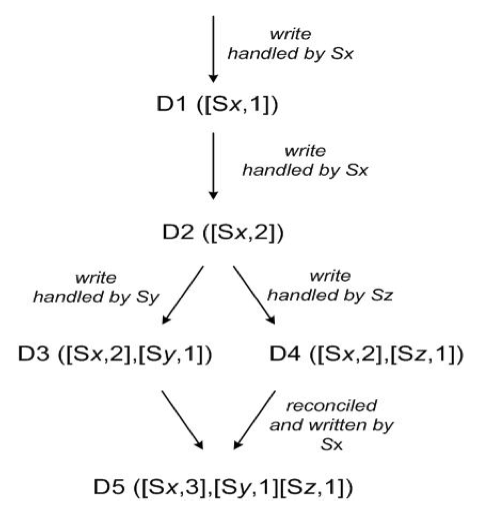
\includegraphics[width=0.7\textwidth]{background/figures/versioning}
    \caption{Version history for an object\cite{voldemort}.}
    \label{fig:versioning}
\end{figure}

To use vector clocks in this manner safely, it is required that all update operations (writes) specify which version we are updating, or we would not be able to infer causality.
This version information must first be obtained through a read of the object, and then passed along with the write.
If during a read the database finds multiple divergent versions of the object, all of the objects at the \emph{end} of the divergent paths are returned.
The application then have to decide what to do, but typically a merged version has to be written. This merged version would specify the union of the versions of its predecessors as its version, creating a merged version.

An example of an objects version history is given in Figure \ref{fig:versioning}. 
The different objects written are labeled DX and the vector clock associated with the object is given in parenthesis. The distinct nodes are designated with S followed by a character, for example $S_x$ and $S_y$ are two distinct nodes.

First a new object, D1 is written to the database. This write is handled by node $S_x$, and it assigns D1 the vector clock \texttt{([$S_x$,1])}.
This is because it is the first version for this key and node $S_x$ managed the write. If another object, D2, is written to the same key is managed by $S_x$, we increment the counter for the $S_x$ version. We then have the object D2 \texttt{([$S_x$,2])}. Note that this means if somewhere we found D1, we could discard D1 if we are also holding D2 because of the versioning causality. D1 is the direct ancestor of D2, and is obsolete.
Next in Figure \ref{fig:versioning}, we have two more objects written to the key, but they are handled by different nodes.
First a client reads D2, then writes object D3. The write of D3 is handled by node $S_y$, with the context from D2. We therefore get the object D3 \texttt{([$S_x$,2],[$S_y$,1])}. We can say D3 \emph{decends} from D2.

Another client has also read D2 earlier. This client writes D4, which coincidentally is also written with the context of D2. D4 ends up being handled by $S_z$. D4 gets the vector clock \texttt{([$S_x$,2],[$S_z$,1])}.

As we can see, D3 and D4 are now on diverging paths, as both are based on D2.
Now when a read happens, either D3 or D4 could be returned, but ideally, and at some point, \emph{both} D3 and D4 will be returned.
The application then needs to perform a \emph{merge}, writing an object, D5, which includes the histories of both D3 and D4.
We see that this indeed occurs, with D5 \texttt{([$S_x$,3],[$S_y$,1],[$S_z$,1])}.

To elaborate, we can see that we will never have to return D2 if we are following vector clocks.
For both D3 and D4, the counter for $S_x$ version for D2 $<= S_x$ for either D3 or D4. We can therefore discard D2 if we have either D3 or D4.

Over time, we can see that the list with vector clocks can grow significantly. Normally only the nodes in the preference list would write new versions of an object, which would be fine. But especially during network partitions, writes can be handled by many different servers not in the preference list for the target partition.
According to Giuseppe DeCandia et al. (Dynamo)\cite{dynamo} they solve this with timestamps. A timestamp is stored with the individual version counters. 
When the number of versions exceeds a number N, the oldest vector clock is deleted.
While this could remove important information and create issues in the database, Giuseppe DeCandia et al.\cite{dynamo} mentions that this problem has never occurred in production.

\subsection{Membership}
In a distributed system individual nodes sometimes need to know whichx other nodes are available in the system. We call this group membership. Whenever a node crashes we want its membership removed so that other nodes are aware of the crash. This can be achieved in various ways. 

\begin{itemize}
\item A central service where nodes register themselves and send keep alive messages to verify that they are alive. When a new member is added or removed the service can simply broadcast a message to all members of the change. A drawback of this strategy is that we now have a single point of failure, as well as a solution that does not scale very well. As we expand and get more nodes in the system, the traffic into the central controller will increase as well. ZooKeeper can be used as one such central service, and we will look at how in the ZooKeeper section.
\item The Gossip Protocol is a decentralized peer-to-peer solution to this problem. Gossip is modeled after how information spreads in social networks. By having nodes pair up with random partners at random intervals to exchange information, we allow information to spread throughout the network. Typically this is membership data, or information about ``\emph{who knows who}'' and what their status is.

For example if Alice discovers Charlie is down, when Bob calls Alice, Alice will tell Bob that Charlie is down.

Gossiping thus allows the system to reach an eventual consistent state without having any \emph{single} broad casted message or a demand for a single up to date catalog of the system state. To add a node to the group, simply pair it with one existing member and let the gossip protocol allow the news of the new node spread. Similarly if a node is unable to pair up with its partner the partner is marked as unreachable and this will be shared with future partners. This approach scales very efficiently as we only have peer to peer communication, but it is not without drawbacks. It is possible to create temporary logical partitions that exists while the information is being spread. Dynamo uses an external system with seed nodes to counteract these logical partitions. 

An example for adding a node with Gossip would be to tell, or \emph{seed} a couple of nodes in the network with information about the newcomer manually. They will then gossip about this new node to their neighbors and the information will gradually spread. In practice this kind of seeding is useful because it really helps propagation go faster. Sometimes these seeding nodes can also be designated as such, and have a larger role in the gossip. One might argue that introducing such hotspots for information is against the pure peer to peer nature of the gossip protocol, but Amazon regards it as necessary to speed up inclusion of new nodes.

\begin{figure}[h]
    \centering
    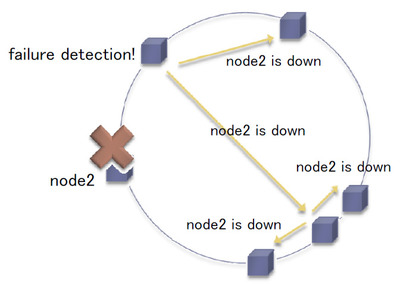
\includegraphics[width=0.5\textwidth]{background/figures/gossip}
    \caption{Gossiping about group membership. A node discovers \texttt{node2} is down, then relays this information to those in his neighbor list.}
    \label{fig:gossip}
\end{figure}


\end{itemize}

\subsection{Failures}
\label{sec:failures}
As we can see, these highly distributed systems are built to allow for failure. We will here explore how Voldemort and Dynamo try to mitigate for failing nodes while also keeping with the operational requirements for consistency and durability. 

\subsubsection{Hinted handoff}
In practice, both nodes and network will fail. During such failures, we still want to continue serving requests.
To satisfy durability during failure, Voldemort perform a form of sloppy quorum. 
Instead of requiring all N members of the quorum to fulfill a durable write, they use temporary hosts. 
By this, we mean that in practice, the N nodes in the preference list a write eventually has to reach, are the next N \emph{healthy} nodes on the ring.
When a node on the preference list is down (marked as not healthy), the request is routed to the next healthy node. 
This write however contains meta data that says who was the intended target for this replica. 
The metadata is then used to push the write back to the intended target once he becomes healthy again.

Looking at Figure \ref{fig:voldemort_hashring}, if a key K hashes to partition 0, the preference list contains nodes \texttt{N0} and \texttt{N1} (recall N=2).
If \texttt{N1} is not responsive, it is not healthy, and assume \texttt{N2} is the next healthy node.
This means that when \texttt{N1} is not responsive, \texttt{N2} is placed on the preference list, because it is the next \emph{healthy} node.
Now when \texttt{N0} receives a write, it will push the replica (to satisfy durability N=2) to \texttt{N2} as long as \texttt{N1} is down.
\texttt{N2} will however receive a write with a hint that this object actually belongs to \texttt{N1}, so \texttt{N2} puts it in a special database to push it to \texttt{N1} at a later time when \texttt{N1} is healthy again. When \texttt{N2} successfully reaches \texttt{N1} and delivers the write, this object is deleted from \texttt{N2}. 
This process is called hinted handoff. 

Using hinted handoff, we can still satisfy durability guarantees during node failures.

\subsubsection{More failures}
Hinted handoff helps in environments with low churn and where nodes usually come back online. But if a node holding a hinted replica goes down before the intended node comes back up, it may even be permanently down and the hinted object is never returned to the intended owner.

To mitigate such permanent failures, Dynamo\cite{dynamo} employs a method to regularly ensure that datasets common between nodes are consistent. A naive approach to this could be sending your entire key set to the other node and compare the data directly.
This is however very costly, both in bandwidth used and is both CPU and disk intensive for both.

To minimize the impact on network load and node performance while simultaneously doing replica synchronization, the database uses hashes of the data. Here Voldemort and Dynamo have different approaches. In Voldemort, each key's hash is sent to the other node for comparison.

In Dynamo, Amazon have implemented merkle trees for comparing data sets between nodes. This significantly reduces workload on a replica synchronization.
A merkle tree is a binary tree of hashes, see Figure \ref{fig:merkletree}, where the leaf nodes are hashes of the key objects.
Now make a hash of the two children nodes.
Then to make the parent node, assign the parent the hash of the two hashes of the children until you have the root node. 

Each node keeps a merkle tree for the keyspace that it shares with the other node. The tree is updated whenever a write is commited.
When a sync happens between two nodes, they only need to compare the value of their root node to know if they have any differences.
One can also see how this method makes it quick to discover which key differs. Each comparison will halve the search area.
I.e. we have a binary search for the differing key or even subtree.

\begin{figure}[h]
    \centering
    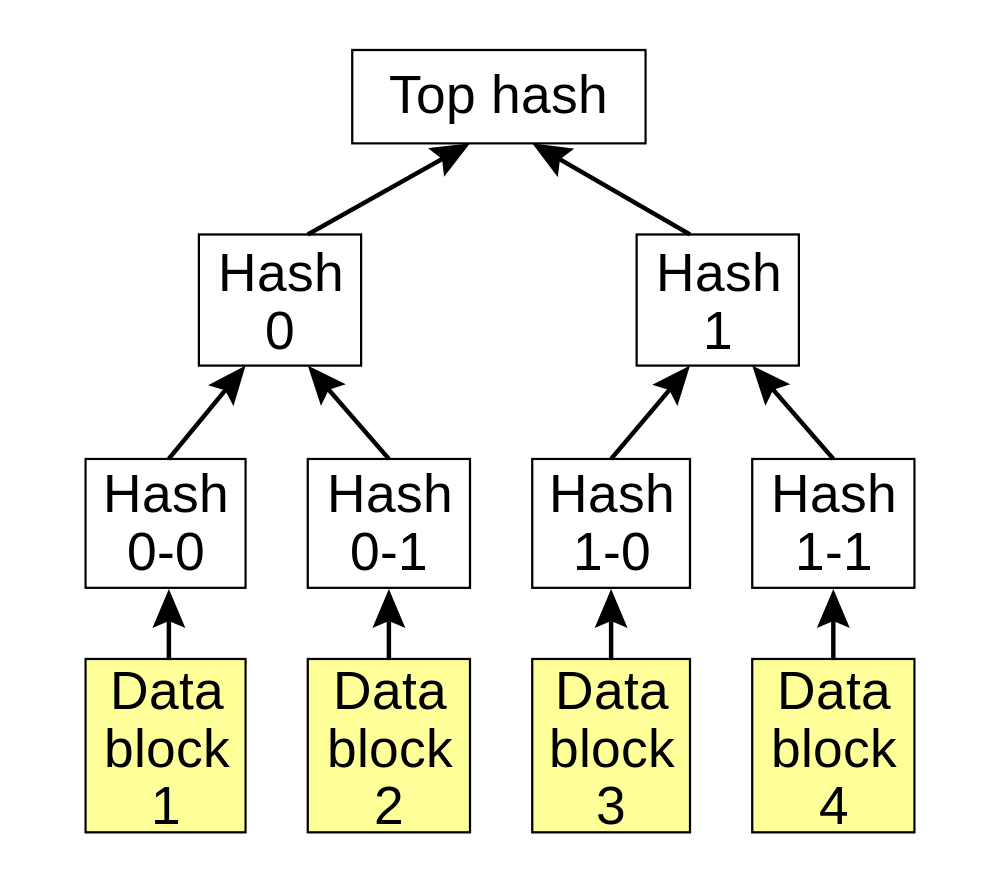
\includegraphics[width=0.5\textwidth]{background/figures/hashtree}
    \caption{Structure of a merkle tree. Notice how the root node can be used for comparing two trees, and how the tree can be used for identifying divergent data.}
    \label{fig:merkletree}
\end{figure}

\subsection{Tunability}
\label{sec:tunability}
As we have briefly outlined above, the database system has three different parameters that are key to operation.
The system gives the admin the opportunity to fine tune certain trade offs after what the implementation needs.

Internally, these are called N, R, W and controls certain aspects of the quorum that is involved in data operations. N is the \emph{eventual} replication factor.
This is the number of nodes we want to store replicas for a key on, and is allowed to happen asynchronously.

\emph{W} is the write factor. This is the number of nodes that synchronously has to be part when we accept a write, and heavily affects performance. 
Typically W is set to two, to make sure an object put must have two replicas in the quorum to be considered successful. 

Another interesting application is the highly writable property store we get with W=1. This means we would never reject a write as long as there is at least one node that can process a request. This will however jeopardize the durability of the data between returning the write and moving the object to other replicas. This setup also has a tendency to introduce a lot more inconsistencies in the data\cite{dynamo}.

The parameter R controls how many nodes must be involved in a read for it to be successful. Setting R low (R=1) would give a high performance read engine. With R=1 though, we might end up with many inconsistencies in the data. It is the read quorum that must decide what data to return. During a read multiple versions of an object might occur. The quorum must then reconcile their versions and return the lastest, or return the conflicting ones.
Because of this, discovering conflicts might be slower when only one node is involved in a read. We are in other words relying on only this single node's world view of the data in a optimistically consistent environment.

Knowing this, when executing a write, the first node to receive the put takes on the role as a coordinator for the write. The coordinator generates the new vector clock and writes a local copy. The coordinator then forwards the request to the top N healthy nodes in the preference list. Nodes that are not healthy are skipped. If W-1 of the healthy nodes report a successful write, the coordinator can return a successful request. 

Reads are handled similarly. The first node receiving the request take on the role as coordinator. The coordinator sends the request to his top N other healthy nodes for the key. After R replies, the coordinator returns the latest version this quorum can agree upon. If there are any divergently versioned objects, all of them are returned to the client for reconciliation.

Amazon\cite{dynamo} mention that their most used configuration for Dynamo is a N=3, W=2, R=2 setup.

\subsection{PAXOS}
Whenever you have a distributed system where errors occur and messages get lost, even simple tasks like deciding on a value can become troublesome. PAXOS is a consensus algorithm made to solve this issue. 

Say we have a set of processes that all can propose values. (The value could be related to leader election). Paxos ensures that a single one of these values is chosen and that all processes involved is notified of this value. If no value is being proposed, then no value should be chosen. 

In Paxos a process can act in three different roles: {\it proposer, acceptor and learner}. A process is not limited to one role at the time. Processes communicate with one another by messages. These messages follow the non-Byzantine model and can take arbitrary long time to be delivered, or they can be lost entirely. They can also be duplicated, however they can not be corrupted. A process acting in a role might also crash, but we assume some critical information will remain through a restart. 

When acting as a proposer, a process will propose a value to a majority subset of acceptors. These acceptors will then accept or deny the proposal according to some rules. Finally if a value is chosen, then all the learners will be informed of this value. The process of choosing a value is given below:

\begin{enumerate}

\item A proposer sends a prepare for proposal message to a majority set of acceptors with a number $n$. This number acts as a timestamp, and represents the last(newest) message this proposer has seen. 
\item Each acceptor receiving this prepare for proposal message will compare the proposed number $n$ with their own highest observed $n$. If the proposed number is higher, then a promise of not accepting any proposal lower than $n$ will be sent back to the proposer along with the acceptors highest observed value. If the proposers number is lower than the acceptors observed number, then the value is sent back along with the highest observed $n$.
\item If the proposer receives a promise from a majority of acceptors, it will send an accept message to the acceptors with the number $n$ along with the value $v$, which is the maximum values received from the acceptors. If the number of promises is less than the majority of acceptors then the attempt has failed, and the proposer must start again with a higher number $n$.
\item When a acceptor receives an accept message, this acceptor will accept this proposal as long as there has not been issued a new proposal with a higher number in the meantime. 
\item Finally, when an acceptor has accepted a proposal it informs all learners. Either by sending a message to all learners, or by sending a message to a designated learner, which in time will inform all other learners. This second step reduces message load but is less reliable.

\end{enumerate}

It is possible to construct a scenario where two proposers keep out proposing each other and no progress is ever made. To combat this a distinguished proposer must be elected. 

Paxos can typically be used in distributed systems to coordinate processes. One example is leader election, another is deciding on the next action to be taken.


